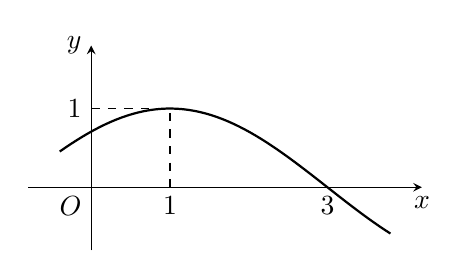
\begin{tikzpicture}[>=stealth, scale=1.0]
  % 坐标轴
  \draw[->] (-0.8, 0) -- (4.2, 0) node[below] {$x$};
  \draw[->] (0, -0.8) -- (0, 1.8) node[left] {$y$};
  \node[below left] at (0, 0) {$O$};

  % 刻度与虚线
  \node[left] at (0, 1) {$1$};
  \node[below] at (1, 0) {$1$};
  \node[below] at (3, 0) {$3$};

  \draw[dashed] (0, 1) -- (1, 1) -- (1, 0);

  % 正弦函数曲线: y = sin(pi/4 * x + pi/4)
  \draw[thick, domain=-0.4:3.8, samples=60] plot (\x, {sin((\x * 0.25 + 0.25) * 180)});
\end{tikzpicture}
